\documentclass[xcolor=dvipsnames,hyperref={pdfpagelabels=false}]{beamer}

\usetheme{Boadilla}

\newcommand{\bi}{\begin{itemize}}
\newcommand{\ei}{\end{itemize}}
\newcommand{\be}{\begin{enumerate}}
\newcommand{\ee}{\end{enumerate}}
\newcommand{\bc}{\begin{center}}
\newcommand{\ec}{\end{center}}
\newcommand{\bd}{\begin{description}}
\newcommand{\ed}{\end{description}}
\newcommand{\I}{\item}
\newcommand{\f}{\frame}
\newcommand{\ft}{\frametitle}

\title{Offline Software Overview}
\subtitle{GlueX Collaboration Meeting}
\author[Mark Ito]{Mark M.\ Ito}
\date{October 3, 2013}
\institute[JLab]{Jefferson Lab}

\begin{document}

\f{\titlepage}

\f{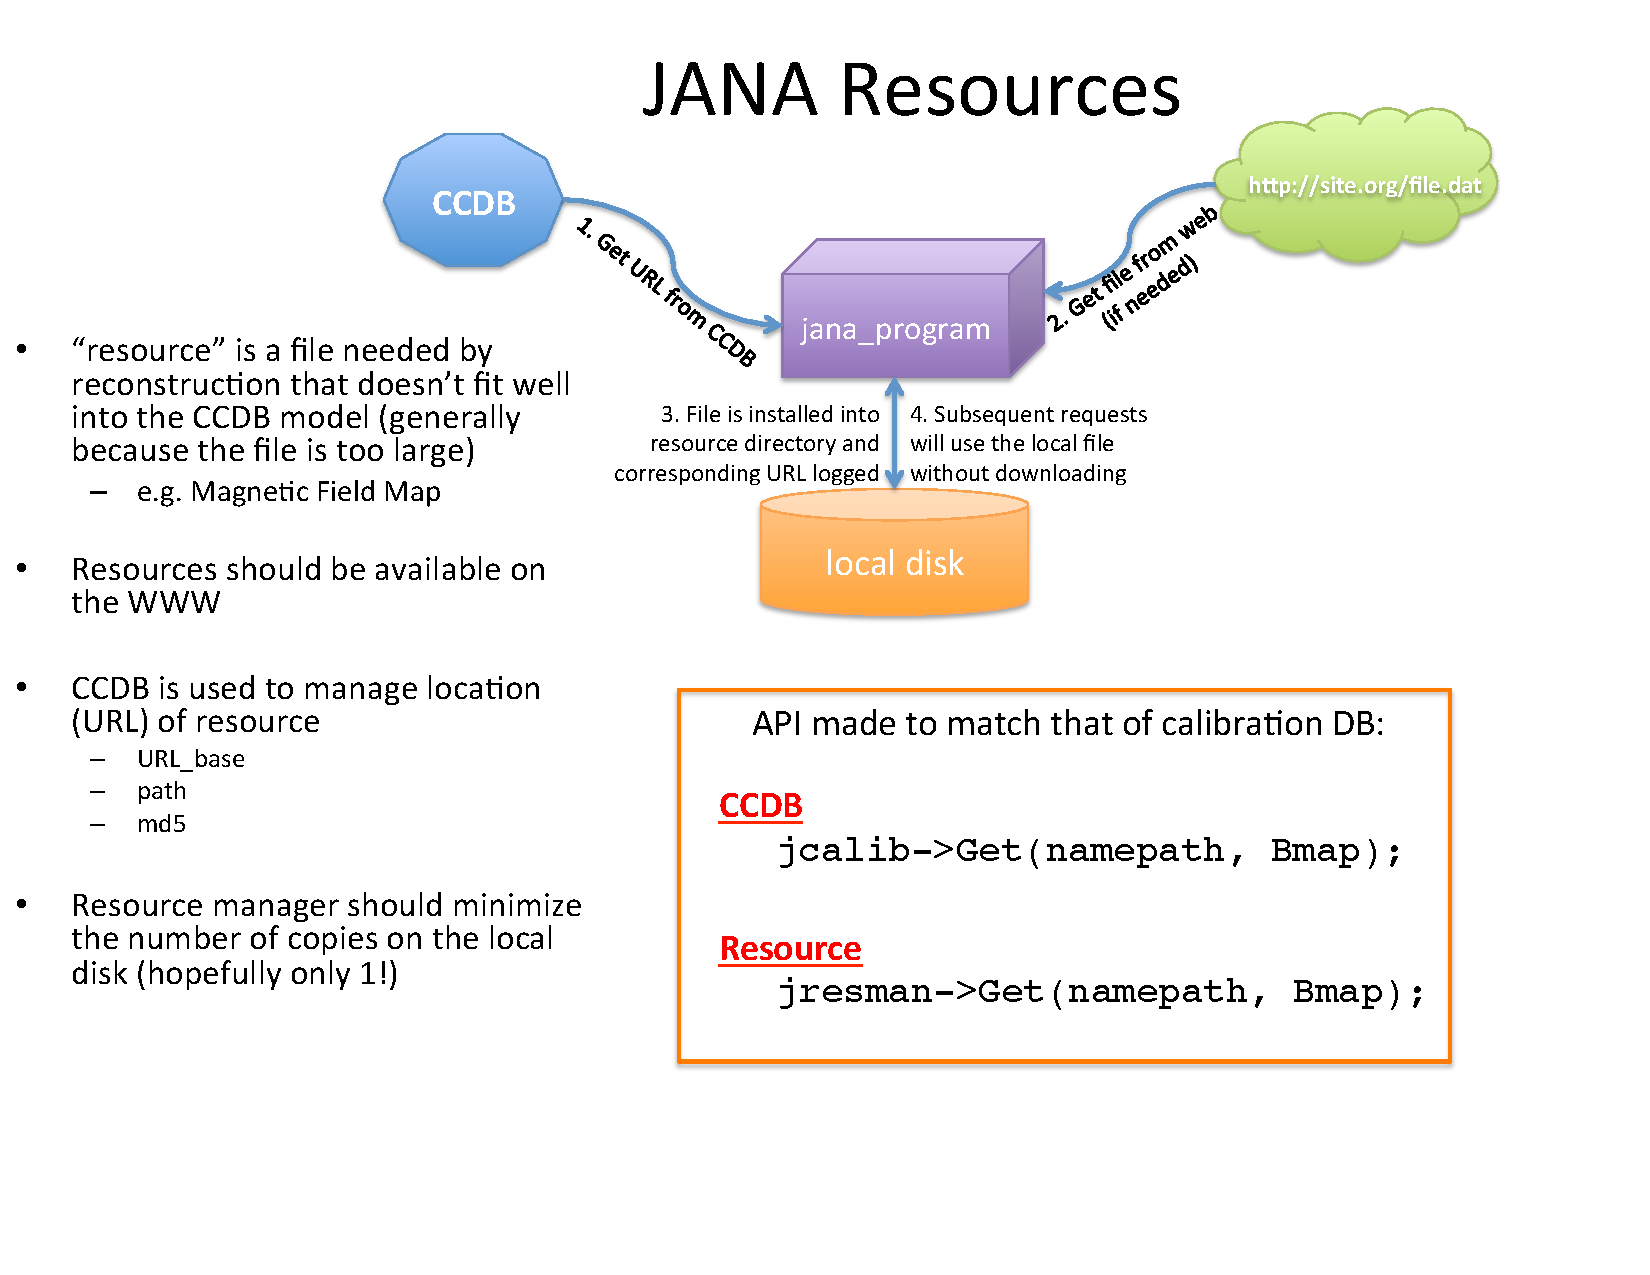
\includegraphics[width=4.5in]{resources.pdf}}

\f{\ft{Other Talks}
\bi
\I analysis workshop
\I BCAL improvements
\I Tracking improvements
\I Online data challenge
\I Software Review
\ei
}

\f{\ft{Top-level build scripts}
  \bi
  \I scripts for installing GlueX software on several flavors of Linux
  \I tested on CentOS 6, Scientific Linux 6, Ubuntu 12.04, Fedora 18, LinuxMint 15, openSUSE 12.3
  \I installation steps
    \be
    \I prerequisites: gluex\_prereq\_<distribution>.sh
    \I subversion test: svn\_touch.sh
    \I install: gluex\_install.sh
    \ee
  \I builds: xerces-c, CERNLIB, ROOT, CLHEP, Geant4, GSL (Gnome Scientific Library), CCDB, JANA, HDDS, sim-recon, and set-up scripts
  \ei
}

\f{\ft{Work Flow}
  \bd
  \I[Work Flow Tools]: standard automation of large-scale, multiple job submission and tracking
  \I[Data Provenance]: having information on how data was processed and archiving tools necessary to re-analyze data in the future.
  \ed
  \bi
  \I SciComp willing to help
  \I Committee formed to set scope
  \I Meetings so far have been educating SciComp staff about issues
  \ei
}

\f{\ft{generated particle and decay chain reporting}
  \bi
  \I Issue: in reconstructed Monte Carlo data want to know the entire particle production, decay, interaction chain
  \I PIC (Pesterer-in-Chief): Kei Moriya
  \I difficulties:
    \be
    \I some action in generator, some in Geant
    \I more than one generator, want uniform scheme
    \I electromagnetic showers produce huge numbers of secondaries, but some of these may be of interest to end user
    \ee
  \I partial solutions implemented
  \I need comprehensive solution, i. e., a design
  \I not high-level rocket science
  \ei
}

\f{\ft{Data Challenge 2}
  \bi
  \I New software
    \bi
    \I fix bugs: improve job success efficiency 
    \I BCAL reconstruction
    \I CCDB
    \I latest tracking
    \I ROOT trees?
    \I improved REST?
    \ei
  \I Simulation Configuration Changes
    \bi
    \I add electromagnetic background
    \I add in dark noise in the BCAL
    \I open up photon window, especially to higher photon energy,
       perhaps 7.5 GeV to the end-point
    \ei
  \I System Improvements
    \bi
    \I farm management system at JLab
      \bi
      \I crude set of perl scripts now, full of kludges
      \I needs generalization, perhaps re-write
      \ei
    \I input and output data cataloging and management
      \bi
      \I database application?
      \I grid-based meta-data catalog?
      \ei
    \ei
  \ei
}
  
\end{document}

We have a data management plan
  meeting with Library School folks from CMU
  same problem as us: funding agencies want to to see this

Data Flow Tools
  at JLab, a requirements document drafted by a committee
  implementation slowed by re-organization
  will not be ready for this data challenge

SCons system for building sim-recon
  in place, in active use
  make system still in place
  some feature discussions going on
    stand-alone libraries

Monte Carlo Genealogy
  scheme that allows family tree to cross over from bggen to hdgeant  

REST Format and Track Swimming
  before: no information on cluster matching to tracks saved
  now: matching information kept in REST format

CCDB
  gateway for access to resources
  closes idle MYSQL connections
  general improvements
    help pages
    better unit testing
    documentation updates
    web-site tweaks
  authentication implemented
  plan for Halls A and C to adopt use

Splitting up the packages
  major categories: simulation, reconstruction, analysis
  other stand-alone candidates: AmpTools, HDDM, ``utilities''
  addresses some issues with old data
  still in planning stage

SQLite versions of CCDB generated automatically, daily

EventStore being explored

Tagged File System for Event Data
  Event distribution
  tags
  filters

Reverse Magnetic Field Fix
  some non-generalities in code exposed
  allows for use of new magntic field with the proper sign

Time-of-Flight Geometry Changes
  added half-width counters

Jana 0.7
  use of resources
  large files
    magnetic fields
    shower shape templates in PbWO$_4$ crystal reconstruction
  local cache
  not a good fit for calibration database
    seldom change, longer characteristic time than normal calibration constants
    local cache a better model
  apply administrative controls
    no deleting resource files once in common use
    robust backup scheme
  use
    environment variable

Geant4
  progress on geometry
  Richard described changes needed last collab meeting due to g4 being pickier than g3
  changes common to both; required for apples-to-apples comparison
  some side-effects of those changes lingered and needed to be been addressed; done now
